%===============================================================================
\section{Traditional beam models}

%===============================================================================
\subsection{Euler-Bernoulli beam theory}

%-------------------------------------------------------------------------------
\begin{frame}
  \frametitle{The Euler-Bernoulli beam (planar case)}
  
  \begin{itemize}
    \item assumption of the model
      \begin{itemize}
        \item all cross sections remain planar
        \item cross section normal and centerline tangent are of same orientation $\varphi$ \newline
          \null \quad $\rightarrow$ model only allows for pure bending (no shear)
      \end{itemize}
    \item bending moment $M(s) = E \, I \, \kappa(s)$
    \item centerline of beam described by function $y(s)$
    \item curvature of centerline given by $\kappa(s) = \frac{\od[2]{y}{s}(s)}{\biggl( 1 + \bigl( \od{y}{s}(s) \bigr)^2 \biggr)^{\frac{3}{2}}}$ \newline
      \null \quad $\rightarrow$ geometric nonlinearity $\rightarrow$ non-linear ODE
    \item linear approximation for small deflections: $\od{y}{s} = \tan(\varphi) \ll 1 \Rightarrow \od{y}{s} \approx \varphi$
    \item Euler-Bernoulli beam equation: $M(s) = E \, I \, \od[2]{y}{s}$
  \end{itemize}
\end{frame}


%-------------------------------------------------------------------------------
\begin{frame}
  \frametitle{Example: Cantilever beam (part 1)}
  
  \begin{figure}
    \centering
    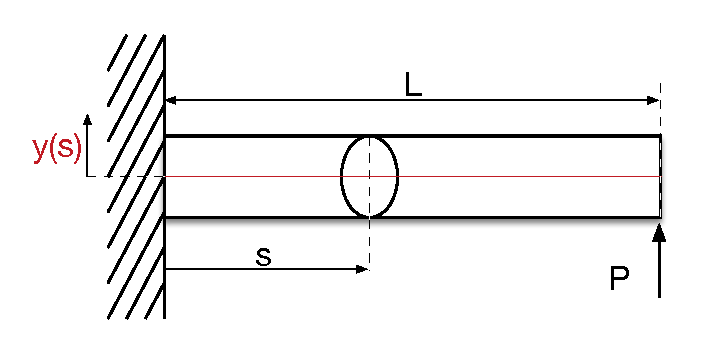
\includegraphics[width=16cm, keepaspectratio=true]{sections/traditional_beams/images/EulerCanitleverExample1part1}
  \end{figure}
  
  \begin{tabularx}{\linewidth}{XX}
    {
      boundary conditions at $s=0$:
      \begin{itemize}
        \item $y(0) = 0$
        \item $\od{y}{s}(0) = 0$
      \end{itemize}
    } & {
      boundary conditions at $s=L$:
      \begin{itemize}
        \item $v(L) = P$
        \item $M(L) = 0 \Rightarrow \od[2]{y}{s}(L) = 0$
      \end{itemize}
    }
  \end{tabularx}
\end{frame}

%-------------------------------------------------------------------------------
\begin{frame}
  \frametitle{Example: Cantilever beam (part 2)}
  
  \begin{figure}
    \centering
    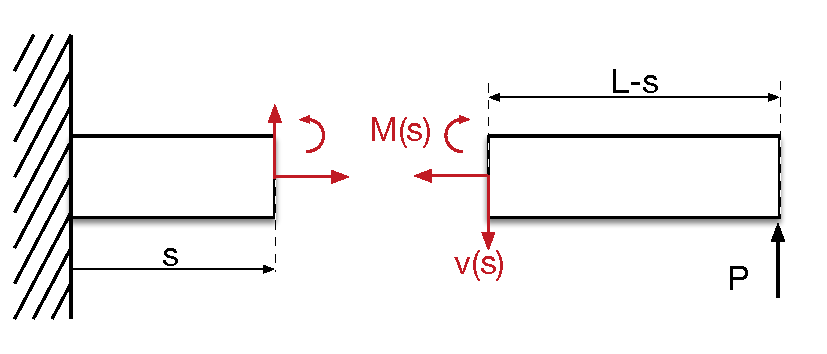
\includegraphics[width=14cm, keepaspectratio=true]{sections/traditional_beams/images/EulerCanitleverExample1part2}
  \end{figure} 
  \vspace{-1.4em}
  
  \begin{displaymath}
  \text{moment balance:} \quad  -M(s) + P(L-s) = 0 \quad \Rightarrow \quad M(s) = P \, (L-s)
  \end{displaymath}
  
  \begin{displaymath}
    M(x) = E \, I \, \od[2]{y}{s} \quad \Rightarrow \quad \od[2]{y}{s} = \frac{M(s)}{E \, I}  = \frac{P \, (L-s)}{E \, I}
  \end{displaymath}
  
  \begin{displaymath}
    \Rightarrow y(s) = \frac{P}{E \, I} \, \biggl( - \frac{s^3}{6} + \frac{L \, s^2}{2} \biggr) + \cancel{c_1} \,s + \cancel{c_2} = \frac{P \, L^3}{2 \, E \, I} \Biggl( \biggl( \frac{s}{L} \biggr)^2 - \frac{1}{3} \biggl( \frac{s}{L} \biggr)^3 \Biggr)
  \end{displaymath}
\end{frame}

%-------------------------------------------------------------------------------
\begin{frame}
  \frametitle{Another example of a cantilever beam}
  
  \begin{figure}
    \centering
    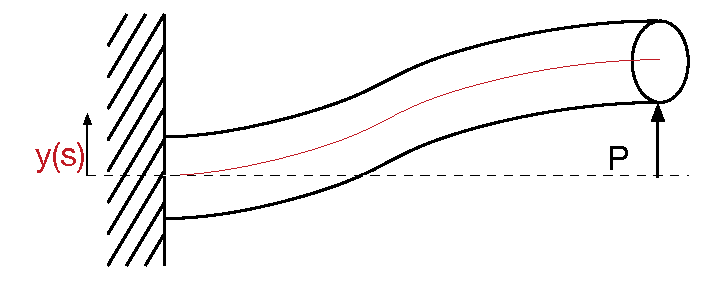
\includegraphics[width=16cm, keepaspectratio=true]{sections/traditional_beams/images/EulerCanitleverExample2}
  \end{figure}
  
  \begin{tabularx}{\linewidth}{XX}
    {
      boundary conditions at $s=0$:
      \begin{itemize}
        \item $y(0) = 0$
        \item $\od{y}{s}(0) = 0$
      \end{itemize}
    } & {
      boundary conditions at $s=L$:
      \begin{itemize}
        \item $v(L) = P$
        \item $\od{y}{s}(L) = 0 \Rightarrow M(L) \neq 0$ \newline
          \null \quad (rotation is restricted)
      \end{itemize}
    }
  \end{tabularx}
  
  \begin{displaymath}
    \Rightarrow M(s) = M(L) + P \, (L-s)
  \end{displaymath}
\end{frame}


%-------------------------------------------------------------------------------
\begin{frame}
  \frametitle{Boundary conditions}
  
  \vspace{4em}
  \begin{center}
    \begin{tabular}{lr}
      displacement & force \\
      \hline
      prescribed $\Rightarrow$ & unknown \\
      unknown & $\Leftarrow$ prescribed \\
      \hline \\
      \\
      rotation & moment \\
      \hline
      prescribed $\Rightarrow$ & unknown \\
      unknown & $\Leftarrow$ prescribed \\
      \hline
    \end{tabular}
  \end{center}
\end{frame}


%===============================================================================
\subsection{Timoshenko beam theory}


%-------------------------------------------------------------------------------
\begin{frame}
  \frametitle{The Timoshenko beam (planar case)}
  
  \vspace{-1em}
  \begin{figure}
    \centering
    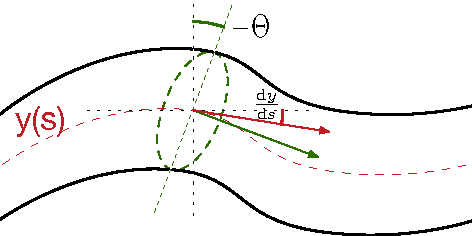
\includegraphics[width=16cm, keepaspectratio=true]{sections/traditional_beams/images/TimoshenkoBeam1}
  \end{figure}
  
  \begin{itemize}
    \item individual cross sections still remain planar
    \item centerline tangent orientation (red) $\neq$ cross section normal (green)
      \begin{itemize}
        \item $-\Theta$ measures orientation of cross section
        \item centerline tangent $\od{y}{s}$ influenced by \textbf{bending and shearing}
      \end{itemize}
    \item shear strain $\gamma(s) = \od{y}{s}(s) - \Theta(s) = \frac{v(s)}{k \, G \, A}$
    \item curvature $\kappa(s) = \od{\Theta}{s}(s) = \frac{M(s)}{E \, I}$ (see next slide)
  \end{itemize}
\end{frame}


%-------------------------------------------------------------------------------
\begin{frame}
  \frametitle{Connection between curvature and moment}

  \begin{multicols}{2}
    \noindent
    
    \begin{figure}
    \centering
      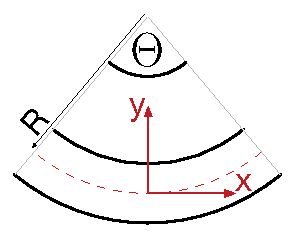
\includegraphics[width=13cm, keepaspectratio=true]{sections/traditional_beams/images/TimoshenkoBeam2}
    \end{figure}
    
    \begin{displaymath}
      L = R \, \Theta \quad \Rightarrow \quad \frac{1}{R} = \frac{\Theta}{L} = \od{\Theta}{s}
    \end{displaymath}
    
    \vspace{0.5em}
    fitting circles to the centerline locally:
    \begin{displaymath}
      \kappa(s) = \od{\Theta}{s}(s)
    \end{displaymath}
    
    \begin{displaymath}
      \epsilon_{xx} = \frac{\Delta L}{L} = \frac{(R-y) \, \Theta - R \, \Theta}{R \, \Theta} = \frac{-y}{R}
    \end{displaymath}
    
    \begin{displaymath}
      \sigma_{xx} = -E \, \frac{y}{R}
    \end{displaymath}
    
    \begin{displaymath}
      M = - \int_{\Omega} y \, \sigma_{xx} \, \dif A = E \, I \, \frac{1}{R} = E \, I \, \kappa
    \end{displaymath}
  \end{multicols}
\end{frame}


%-------------------------------------------------------------------------------
\begin{frame}
  \frametitle{Bending and axial compression together}

  \begin{multicols}{2}
    \noindent
    
    \begin{figure}
    \centering
      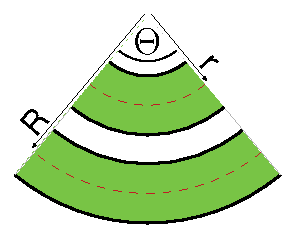
\includegraphics[width=13cm, keepaspectratio=true]{sections/traditional_beams/images/TimoshenkoBeam3}
    \end{figure}
      
    Because of axial forces the beam got shorter!
    \begin{displaymath}
      \begin{alignedat}{1}
        \epsilon_{xx} &= \frac{(r-y) \, \Theta - R \, \Theta}{R \, \Theta} = \frac{r-R}{R} + \frac{-y}{R} \\ 
        &= \epsilon - \frac{y}{R}
      \end{alignedat}
    \end{displaymath}
    
    \vspace{0.2em}
    stress due to axial stretch + bending:
    \begin{displaymath}
      \sigma_{xx} = E \, \bigl( \epsilon + \frac{-y}{R} \bigr)
    \end{displaymath}
    
    \vspace{-0.7em}
    \begin{displaymath}
      \begin{alignedat}{1}
        M &= - \int_{\Omega} y \, \sigma_{xx} \, \dif A \\
          &= - E \, \epsilon \cancel{\int_{\Omega} y \, \dif A} + \frac{E}{R} \int_{\Omega} y^2 \dif A \\ 
          &= E \, I \, \kappa
      \end{alignedat}
    \end{displaymath}
    
    $\rightarrow$ Bending and axial stretch are independent!
  \end{multicols}
\end{frame}


%-------------------------------------------------------------------------------
\begin{frame}
  \frametitle{Model linearity}
  
  \begin{displaymath}
    \begin{alignedat}{1}
      \od{y}{s} &= \frac{1}{k \, G \, A} \cdot v(s) + \Theta  \\ \\
      \od{\Theta}{s} &= \frac{1}{E \, I} \cdot M(s)
    \end{alignedat}
  \end{displaymath}

  \vspace{1em}
  We obtained a linear model because we assumed...
  \begin{itemize}
    \item small slopes of the centerline (linear kinematics)
      \begin{itemize}
        \item $\od{y}{s} = \tan{\Theta} \approx \Theta$
        \item approximation is not valid for larger deformations
      \end{itemize} 
    \item material linearity (linear constitutive law)
      \begin{itemize}
        \item $v(s)$, $M(s)$ get multiplied by constants \newline
          or by functions that depend on $s$ but not on $v(s)$, $M(s)$
        \item material may eg. get stiffer with increasing deformation energy
        \item btw. $k$ is a correction factor, that depends on the shape of the beam's cross section
      \end{itemize}
  \end{itemize}
\end{frame}

%-------------------------------------------------------------------------------
\begin{frame}
  \frametitle{Example: Cantilever beam (part 1)}
  
  \begin{figure}
    \centering
    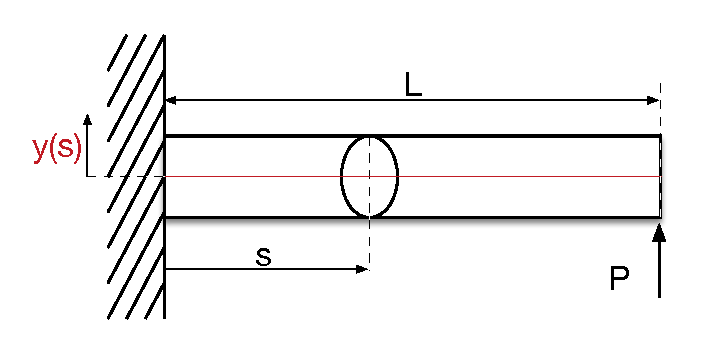
\includegraphics[width=16cm, keepaspectratio=true]{sections/traditional_beams/images/EulerCanitleverExample1part1}
  \end{figure}
  
  \begin{tabularx}{\linewidth}{XX}
    {
      Boundary conditions at $s=0$:
      \begin{itemize}
        \item $y(0) = 0$
        \item $\xcancel{\od{y}{s}(0) = 0}$ (because of shear!)
        \item $\Theta(0) = 0$ (cross section fixed)
      \end{itemize}
    } & {
      Boundary conditions at $s=L$:
      \begin{itemize}
        \item $v(L) = P$
        \item $M(L) = 0$
      \end{itemize}
    }
  \end{tabularx}
\end{frame}

%-------------------------------------------------------------------------------
\begin{frame}
  \frametitle{Example: Cantilever beam (part 2)}
  
  As before with the Euler-Bernoulli cantilever beam we have
  \begin{displaymath}
    v(s) = P \quad \text{ and } \quad M(s) = P \, (L-s)
  \end{displaymath}
  
  \vspace{1em}
  We integrate the Timoshenko beam equations ...
  \vspace{0.3em}
  \begin{displaymath}
    \od{\Theta}{s}(s) = \frac{M(s)}{E \, I} = \frac{P \, (L-s)}{E \, I}
    \quad \Rightarrow \quad
    \Theta(s) = \frac{P}{E \, I} \biggl( L \, s - \frac{s^2}{2} \biggr) + \cancel{c}
  \end{displaymath}
  
  \vspace{1em}
  
  \begin{displaymath}
    \od{y}{s}(s) = \frac{v(s)}{k \, G \, A} + \Theta(s) = \frac{P}{k \, G \, A} + \frac{P}{E \, I} \biggl( L \, s - \frac{s^2}{2} \biggr)
  \end{displaymath}
  
  \begin{displaymath}
    \Rightarrow y(s) = \frac{P \, s}{k \, G \, A} + \frac{P}{E \, I} \biggl( L \frac{s^2}{2} - \frac{s^3}{6} \biggr) + \cancel{c} = \frac{P \, s}{k \, G \, A} + \frac{P \, L^3}{2 \, E \, I} \Biggl( 
      \biggl( \frac{s}{L} \biggr)^2 - \frac{1}{3} \biggl( \frac{s}{L} \biggr)^3 \Biggr)
  \end{displaymath}
\end{frame}


%-------------------------------------------------------------------------------
\begin{frame}
  \frametitle{Comparison of Euler-Bernoulli and Timoshenko cantilever beams}
  
  \textbf{Euler-Bernoulli beam}
  \begin{displaymath}
    y^{(E)}(s) = \frac{P \, L^3}{2 \, E \, I} \Biggl( \biggl( \frac{s}{L} \biggr)^2 - \frac{1}{3} \biggl( \frac{s}{L} \biggr)^3 \Biggr)
    \Rightarrow y^{(E)}(L) = \frac{P \, L^3}{3 \, E \, I}
  \end{displaymath}
  
  \textbf{Timoshenko beam}
  \begin{displaymath}
    y^{(T)}(s) = \frac{P \, s}{k \, G \, A} + \frac{P \, L^3}{2 \, E \, I} \Biggl( 
      \biggl( \frac{s}{L} \biggr)^2 - \frac{1}{3} \biggl( \frac{s}{L} \biggr)^3 \Biggr)
      \Rightarrow y^{(T)}(L) = \frac{P \, L}{k \, G \, A} + \frac{P \, L^3}{3 \, E \, I}
  \end{displaymath}
  
  \textbf{relative error} (taking Euler-Bernoulli as the reference)
  \begin{displaymath}
    \begin{alignedat}{1}
      \epsilon_r &= \frac{y^{(T)}(L) - y^{(E)}(L)}{y^{(E)}(L)} = \frac{\frac{P \, L}{k \, G \, A}}{\frac{P \, L^3}{3 \, E \, I}} = \frac{3 \, E \, I}{k \, G \, A \, L^2} \\
      &= \frac{3 \, E \, b \, h^3}{k \, G \, b \, h \, L^2 \, 12} = \frac{1}{4} \frac{E}{k \, G} \biggl( \frac{h}{L} \biggr)^2
    \end{alignedat}
  \end{displaymath}
  
  \begin{center}
    $\rightarrow$ Euler-Bernoulli beam model performs equally good as the Timoshenko model \newline when the beam is very slender ($h/L$ small)
  \end{center}
\end{frame}


%-------------------------------------------------------------------------------
\begin{frame}
  \frametitle{Another example of a cantilever beam (part 1)}
  
  \vspace{-0.7em}
  \begin{figure}
    \centering
    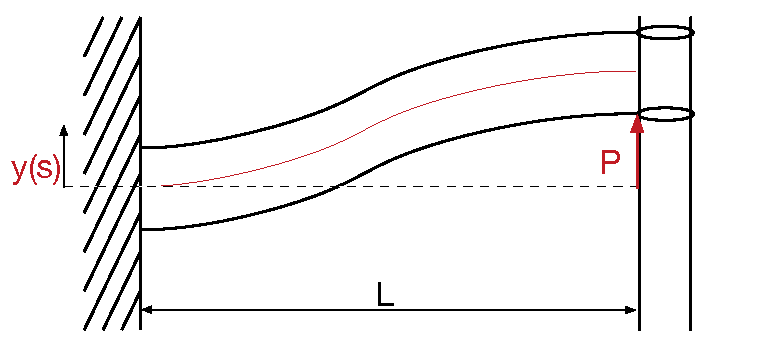
\includegraphics[width=16cm, keepaspectratio=true]{sections/traditional_beams/images/TimoshenkoCanitleverExample2part1}
  \end{figure}
  \vspace{-0.5em}
  cross section at $s=L$ can not rotate or displace horizontally
  \vspace{1em}
  
  \begin{tabularx}{\linewidth}{XX}
    {
      boundary conditions at $s=0$:
      \begin{itemize}
        \item $y(0) = 0$
        \item $\Theta(0) = 0$
      \end{itemize}
    } & {
      boundary conditions at $s=L$:
      \begin{itemize}
        \item $v(L) = P$
        \item $\Theta(L) = 0$
      \end{itemize}
    }
  \end{tabularx}
\end{frame}


%-------------------------------------------------------------------------------
\begin{frame}
  \frametitle{Another example of a cantilever beam (part 2)}
  
  \vspace{-0.7em}
  \begin{figure}
    \centering
    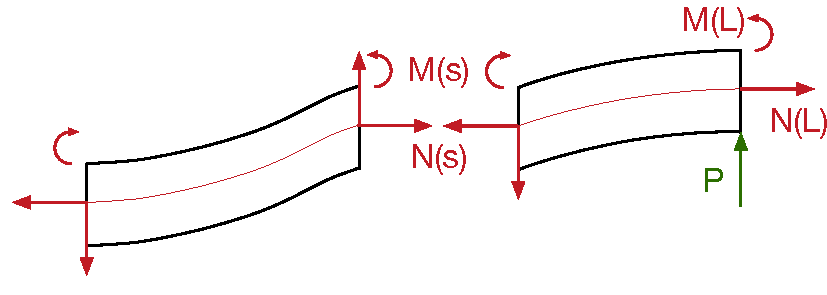
\includegraphics[width=20cm, keepaspectratio=true]{sections/traditional_beams/images/TimoshenkoCanitleverExample2part2}
  \end{figure}
  
  moment balance (in the deformed configuration):
  \begin{displaymath}
    -M(s) + M(L) + P \, (L-s) - N(y(L)-y(s))
  \end{displaymath}
  $\rightarrow$ the last term results in nonlinear behavior of the model \newline
  $\rightarrow$ $M(L)$ and $N(L)$ are two extra unknowns
\end{frame}